%TCIDATA{LaTeXparent=0,0,relatorio.tex}
 


\chapter{Introdução}

\label{CapIntro}

% Resumo opcional. Comentar se não usar.
\resumodocapitulo{A motivação do presente trabalho aparece na área petrolífera, nas operações de reentrada de risers e o objetivo é a validação de um sistema de controle em malha fechada em escala laboratorial como uma alternativa ao modelo manual empregado atualmente.}


\section{Contextualização}

O petróleo tem importância econômica global. Uma das formas de extração do mesmo é aquela feita em águas profundas, a qual o Brasil tem feito importantes avanços desde a descoberta do Pré-Sal em 2006. Em abril de 2015, chegou-se à produção de mais de 800 mil barris por dia no pré-sal, com campos situados em águas profundas e ultraprofundas \cite{preSal}. Os desafios nesta área da engenharia são enormes, pois as operações são muito complexas.

Na Figura \ref{riser}, observa-se uma das operações necessárias para a extração no Pré-Sal, especificamente a operação de reentrada. Nesta operação, um \textit{riser} deve ser conectado da plataforma até o poço de petróleo no leito oceânica. O comprimento do \textit{riser} chega a 2km.

Devido à complexidade inerente das diversas operações \textit{offshore}, propulsores e sensores de localização e orientação - GPS, giroscópios, câmeras, etc - são requisitos essenciais para se poder posicionar a embarcação e os \textit{risers} \cite{redytton}.

\begin{figure}[ht!]
\centering
  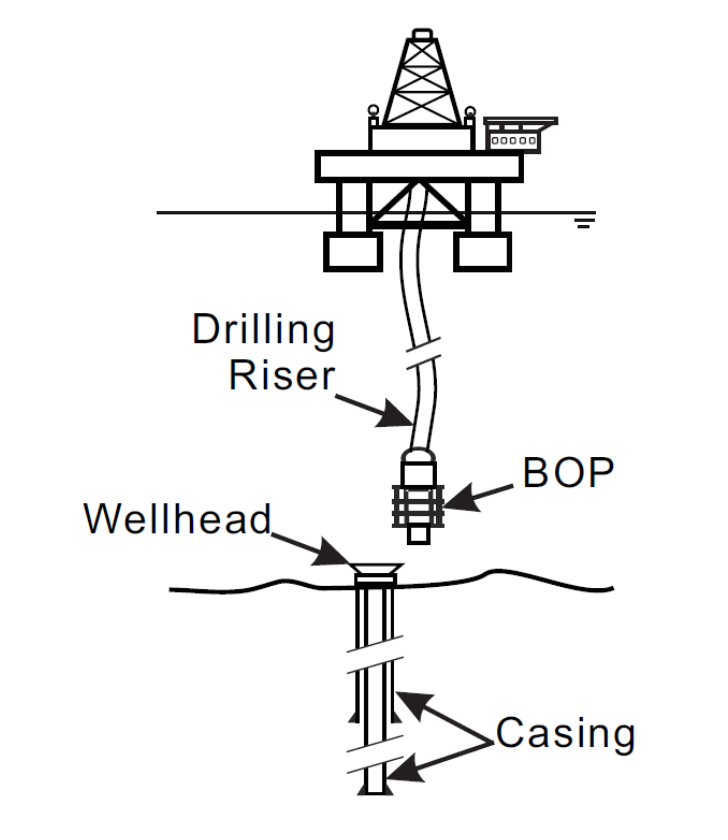
\includegraphics[width=5cm]{figs/introducao/riser}
  \caption{Operação de reentrada \cite{eugenioASME2012}\label{riser}}
\end{figure}


\section{Objetivos do projeto}

O foco deste trabalho está na operação de reentrada, conforme apresentada na Figura \ref{riser}. Atualmente, é uma operação feita manualmente por um operador na plataforma que observa remotamente as imagens capturas por \textit{ROV}s (\textit{Remotely Operated Vehicles}) da região do \textit{riser} próxima ao poço e controla a plataforma através de um \textit{joystick} com o auxílio do sistema de posicionamento dinâmico. O custo envolvido na operação é enorme e os riscos para o equipamento também, já que os próprios \textit{ROVs} e o \textit{riser} ficam sujeitos às perturbações das ondas, correntezas e variações ambientais no fundo do mar. A Figura \ref{posicionamentoAtual} apresenta o esquema que acabou de ser descrito.

\begin{figure}[ht!]
\centering
  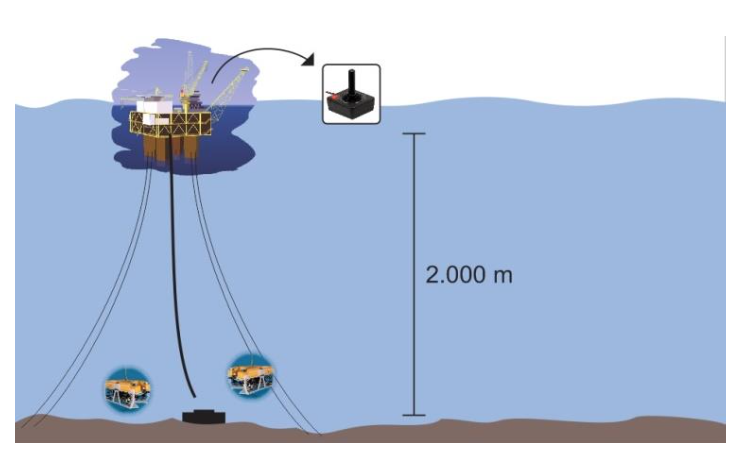
\includegraphics[width=7cm]{figs/introducao/posicionamentoAtual}
  \caption{Método atual para reconexão no poço \cite{redytton} \label{posicionamentoAtual}}
\end{figure}

O objetivo deste trabalho é apresentar uma forma mais eficiente de realizar a operação de reentrada, economizando tempo e recursos, evitando riscos para pessoal e equipamento. Rédytton \cite{redytton} validou o controle em malha aberta. Neste presente trabalho, deseja-se revalidar a malha aberta, com pequenas mudanças na excursão total do carrinho em comparação com o trabalho de Rédytton, assim como realizar as configurações necessárias para fechar a malha.

\begin{figure}[ht!]
\centering
  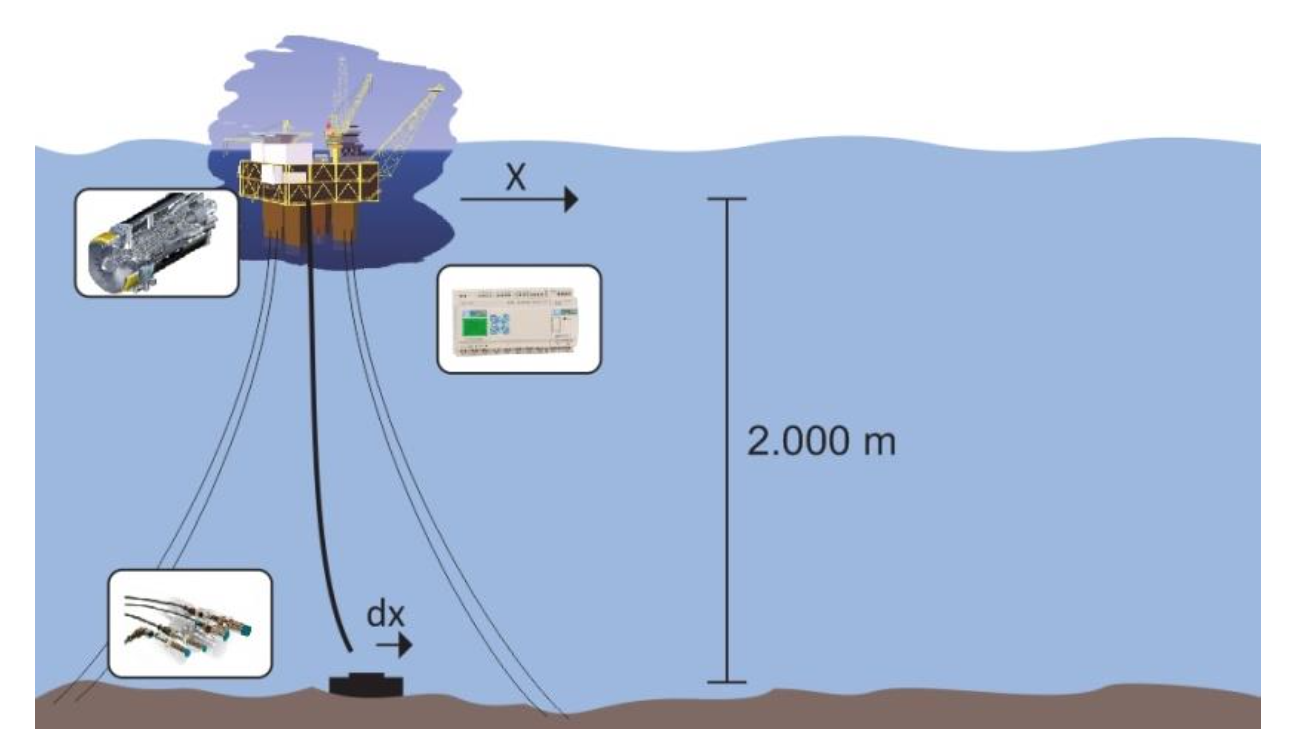
\includegraphics[width=7cm]{figs/introducao/posicionamentoProposto}
  \caption{Método proposto para reconexão no poço \cite{redytton} \label{posicionamentoProposto}}
\end{figure}

Para fechar a malha, necessita-se de um sensor que realimente os dados de posição, o qual, na presente bancada, é uma câmera industrial. Passos necessários incluem: \begin{itemize}
	\item Alimentação da câmera;
	\item Atualização do Firmware da Câmera
	\item Conexão na rede Ethernet/IP da câmera e CLP;
	\item Configuração da câmera no software RSLogix;
	\item Alimentação da bancada com fontes dedicadas de 24V\footnote{Anteriormente, duas fontes de tensão de saída ajustável eram utilizadas, mas foram trocadas por fontes de saída de tensão única.}
\end{itemize}

